\documentclass{article}
\usepackage[utf8]{inputenc}
\usepackage{graphicx}
\usepackage{geometry}
\usepackage{amsmath}
\usepackage{amsfonts}
\usepackage{float}
\usepackage{caption}
\usepackage{subcaption}
\usepackage{enumitem}

\geometry{left=25mm, top=25mm, right=25mm, bottom=25mm}

\title{PHY407 Lab 5}
\author{Pierino Zindel (1002429703) and Hayden Johnson (1002103537)}
\date{October 12, 2018}

\begin{document}

\maketitle

\noindent \textbf{Distribution of work:} Question 1 parts a through c were completed by Hayden. Question 1 part d and question 2 were completed by Pierino.

\section{Basic Applications of the Fourier Transform}

\subsection{a) Newman 7.2: Detecting Periodicity}

\subsubsection{Part a)}

We seek to plot the data contained in the file sunspots.txt and estimate the period of the cyclic component of the data.

A plot of the sunspot data is shown in figure \ref{fig:1a_timeseries}, from which it is clear that there is a regular cycle of fluctuations present in the data. A zoomed in section is shown in figure \ref{fig:1a_timeseries_zoom}, from which it can bee seen that the period of the cycle is roughly:
\begin{align*}
	T &\approx \frac{2970 - 2590}{3} \\
	&\approx 127 \text{months}
\end{align*}

\begin{figure}[H]
	\centering
	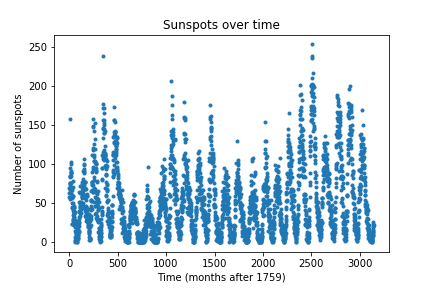
\includegraphics[width=0.8\textwidth]{../images/1a_timeseries.png}
	\caption{Plot showing the number of observed sunspots over time.}
	\label{fig:1a_timeseries}
\end{figure}

\begin{figure}[H]
	\centering
	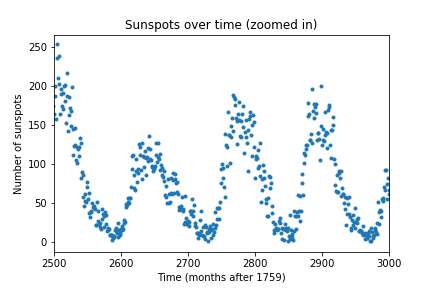
\includegraphics[width=0.8\textwidth]{../images/1a_timeseries_zoomed.png}
	\caption{Zoomed in section of figure \ref{fig:1a_timeseries}.}
	\label{fig:1a_timeseries_zoom}
\end{figure}

\subsubsection{Part b)}

We want to calculate the power spectrum of the sunspot data, and plot it.

The Fourier coefficients of the sunspot data were calculated using np.fft.rfft(), and then the magnitude squared of the coefficients was calculated using np.abs(), which computes the magnitude of a complex number, and squaring this result. A plot of the power spectrum is shown in figure \ref{fig:1a_fourier}. A zoomed in plot of the relevant features is shown in figure \ref{fig:1a_fourier_zoom}, from which it can be seen that there is a clear peak at a non-zero value of $k$.

\begin{figure}[H]
	\centering
	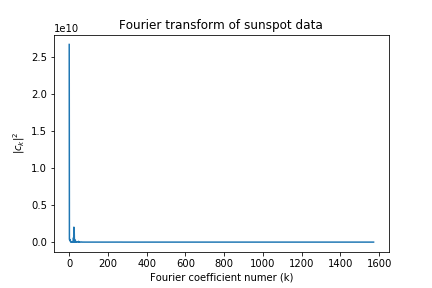
\includegraphics[width=0.8\textwidth]{../images/1a_fourier.png}
	\caption{Fourier transform of the data shown in figure \ref{fig:1a_timeseries}.}
	\label{fig:1a_fourier}
\end{figure}

\begin{figure}[H]
	\centering
	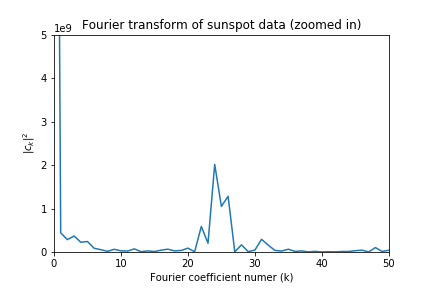
\includegraphics[width=0.8\textwidth]{../images/1a_fourier_zoomed.png}
	\caption{Zoomed in section of figure \ref{fig:1a_fourier}.}
	\label{fig:1a_fourier_zoom}
\end{figure}

\subsubsection{Part c)}

We would like to determine the number of the Fourier coefficient at which the peak occurs, and figure out what period of sine wave corresponds to this number coefficient.

As can be seen from figure \ref{fig:1a_fourier_zoom}, the peak in the Fourier transform occurs at the coefficient with $k\approx 24$. The frequency that corresponds to this number coefficient is:
\begin{equation*}
	f = \frac{k}{L}
\end{equation*}
where $L = 3143$ is the length of the interval covered by the data. Thus, the period is:
\begin{equation*}
	T = \frac{L}{k} = \frac{3143}{24} \approx 131 \text{months}
\end{equation*}
This is in fairly good agreement with the value of $T\approx 127$ months that we found by eye in part a), as we should expect it to be.

\subsection{b) Newman 7.4: Fourier Filtering and Smoothing}

\subsubsection{Part a)}

We seek to read the data from dow.txt and plot it.

This was done using np.loadtxt() and matplotlib.pyplot. The graph produced is shown in figure \ref{fig:1b_dow}.

\begin{figure}[H]
	\centering
	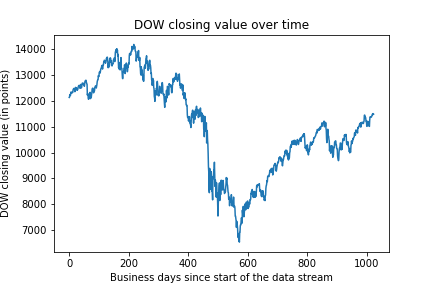
\includegraphics[width=0.8\textwidth]{../images/1b_dow.png}
	\caption{Plot of the DOW closing value (in points) as a function of business days since the start of the data stream (in ``late 2006").}
	\label{fig:1b_dow}
\end{figure}

\subsubsection{Part d) \& e)}

After computing the Fourier transform of the DOW data and then setting the last 90\% of the coefficients to zero, we then want to compute the inverse Fourier transform of the filtered Fourier coefficients and plot this on the same graph as the original data.

\begin{figure}[H]
	\centering
	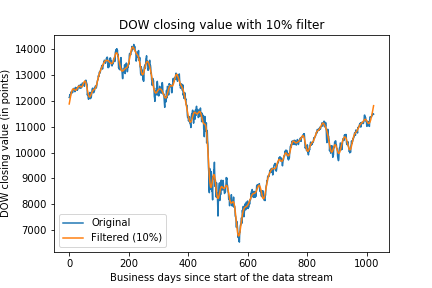
\includegraphics[width=0.8\textwidth]{../images/1b_filtered_10.png}
	\caption{Plot of DOW closing value data along with the filtered version of the data, which was generated by keeping the first 10\% of the Fourier coefficients and setting the rest to zero, as described in the text.}
	\label{fig:1b_filtered_10}
\end{figure}

The filtering of the data was achieved by taking the Fourier transform of the DOW data, and then setting the last 90\% of the coefficients to zero, and finally using np.fft.irfft() to take the inverse Fourier transform of the filtered coefficients, as suggested. This filtered inverse Fourier transform is plotted along with the original data in figure \ref{fig:1b_filtered_10}. The higher number Fourier coefficients correspond to higher frequency components of the data when viewed as a periodic function. We see from the graph that by manually setting these higher frequency components to zero, the small-scale fluctuations in the data are smoothed over, so to speak, and the filtered function traces over the general shape of the original data while ignoring the quick deviations from the general trend. Indeed, we see that applying an even stronger filter of keeping only the first 2\% of coefficients non-zero takes the smoothing even farther, as seen in figure \ref{fig:1b_filtered_02}, with the filtered function ignoring even moderately sized peaks and troughs in the data and just tracing out an average value of sorts.

\begin{figure}[H]
	\centering
	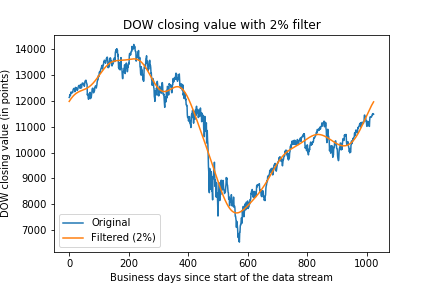
\includegraphics[width=0.8\textwidth]{../images/1b_filtered_02.png}
	\caption{Plot of DOW closing value data along with the filtered version of the data, which was generated by keeping the first 2\% of the Fourier coefficients and setting the rest to zero, as described in the text.}
	\label{fig:1b_filtered_02}
\end{figure}

\subsection{c) Newman 7.6: Comparison of the DFT and DCT}

\subsubsection{Part a)}

We want to write a program analogous to that of part e) of Newman 7.4, which extracts data from the dow2.txt file, takes the Fourier transform of it, sets all but the first 2\% of the Fourier coefficients to be zero, and then takes the inverse Fourier transform of the filtered coefficients and plots both this and the original data.

The data from dow2.txt were extracted, the Fourier transform taken, the last 98\% of the coefficients set to zero, the inverse Fourier transform taken, and the filtered and original data plotted in figure \ref{fig:1c_dft}, just as was done in part e) of Newman 7.4. As can be seen from the plot in figure \ref{fig:1c_dft}, the filtered data does a fairly good job of tracking the general shape of the original data across most of the domain, but it deviates considerably from the original at the endpoints. This is exactly the expected behaviour described in Newman, which occurs as a result of the fact that the Fourier transform requires the function to be periodic, and by throwing away the high-frequency coefficients, we have limited the ability of the function to jump very quickly between the two values which it would like to take at the endpoints, and instead it must traverse the gap more gradually.

\begin{figure}[H]
	\centering
	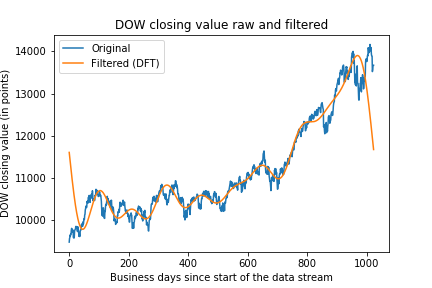
\includegraphics[width=0.75\textwidth]{../images/1c_dft.png}
	\caption{Plot showing DOW closing value data from 2004 to 2008, as well as a smoothed version of the data calculated by setting all but the first 2\% of the coefficients of the discrete Fourier transform to be zero and taking the inverse discrete Fourier transform of this filtered set of coefficients.}
	\label{fig:1c_dft}
\end{figure}

\subsubsection{Part b)}

We seek to repeat part a), but instead of using the discrete Fourier transform, using the discrete cosine transform, in order to avoid the undesirable behaviour of the filtered function near the endpoints.

\begin{figure}[H]
	\centering
	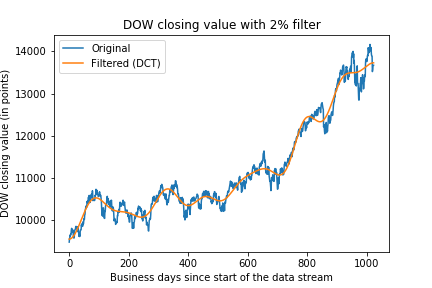
\includegraphics[width=0.75\textwidth]{../images/1c_dct.png}
	\caption{Plot showing DOW closing value data from 2004 to 2008, as well as a smoothed version of the data calculated by setting all but the first 2\% of the coefficients of the discrete cosine transform to be zero and taking the inverse discrete cosine transform of this filtered set of coefficients.}
	\label{fig:1c_dct}
\end{figure}

Using the functions for the discrete cosine transform and the inverse discrete cosine transform included in the file dcst.py provided online by Newman, the code from part a) was modified to compute the discrete cosine transform of the original data, set all but the first 2\% of these coefficients to be zero, and then take the inverse discrete cosine transform of the filtered coefficients to produce a smoothed version of the function. The result is plotted in figure \ref{fig:1c_dct}, from which it can be seen that the filtered function does indeed match the original data much better near the endpoints than the filtered function obtained from the discrete Fourier transform of the same data with the same fraction of non-zero coefficients. As discussed in Newman, this result is expected because, unlike the discrete Fourier transform, the discrete cosine transform does not require the value of the function to be the same at both endpoints.

\subsection{d) Newman 7.3: Musical Instruments}
For this question we aim to take waveform data, provided via Newman's Computational Physics site, for two instruments, a piano and a trumpet, and perform a Fourier transform on the data sets to retrieve the initial note played on each instruments. 

\subsubsection{Part a)}

\begin{figure}[H]
	\centering
	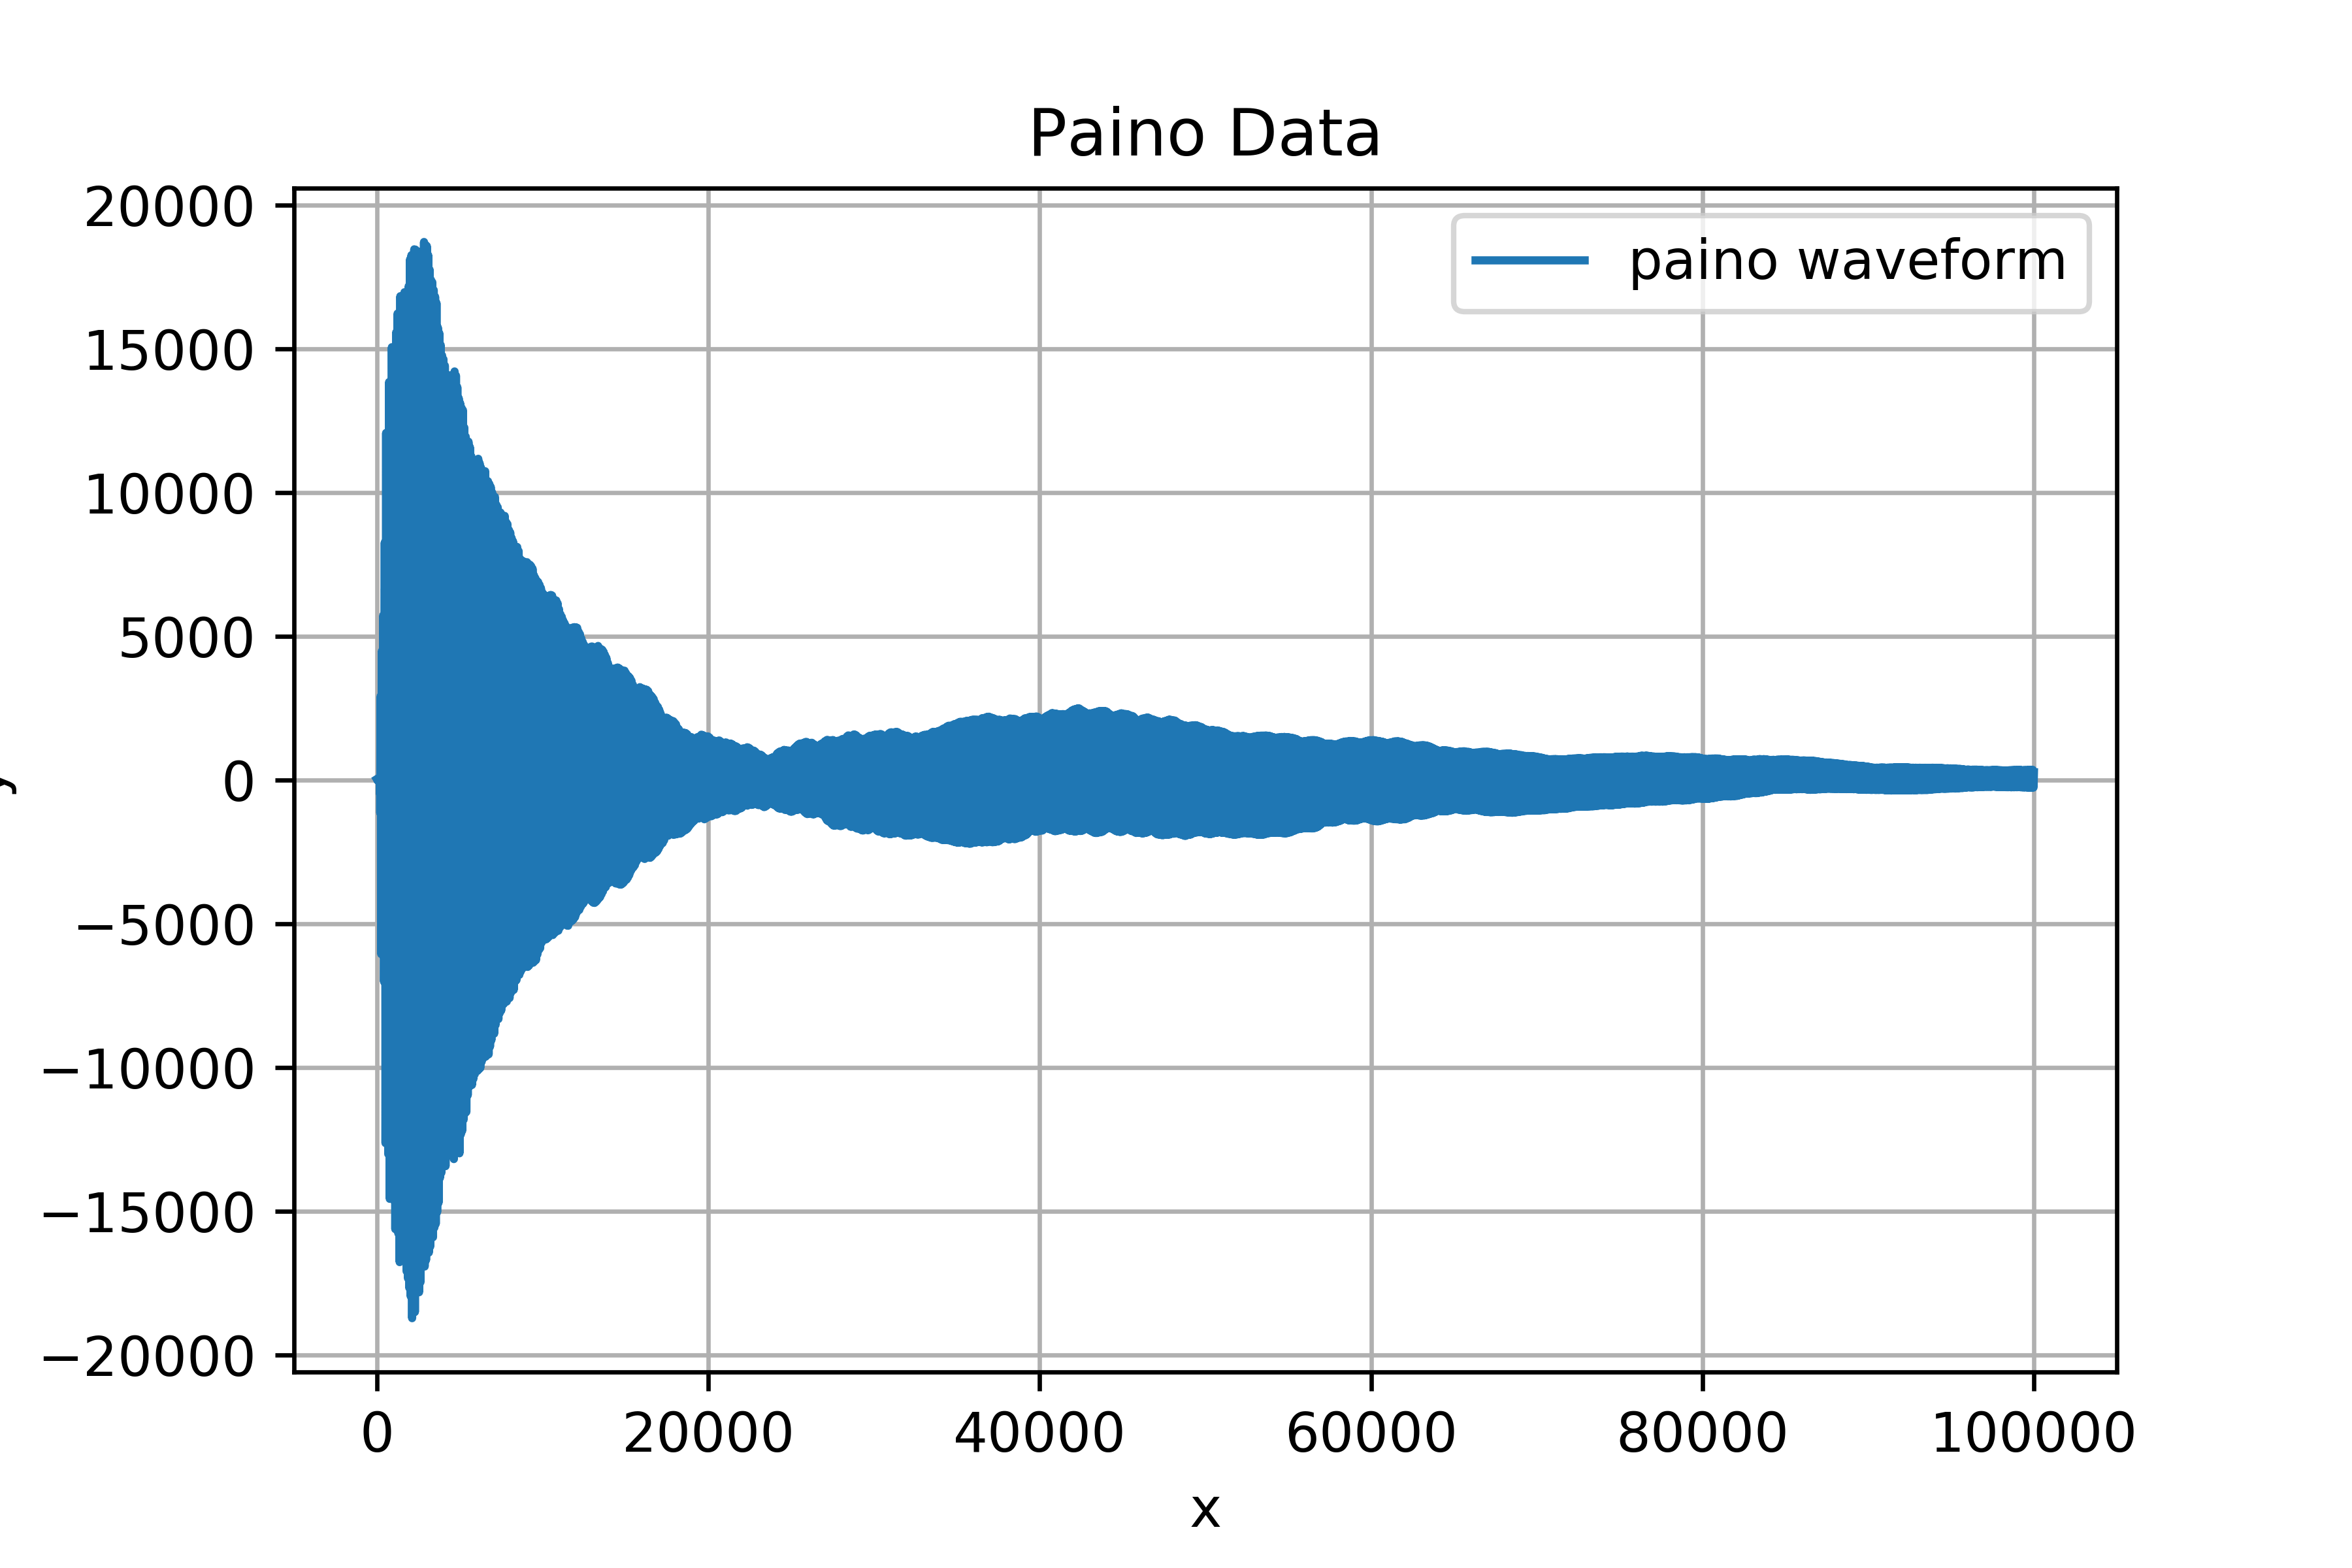
\includegraphics[width=0.8\textwidth]{../images/piano_wave.png}
	\caption{Plot of the waveform for a note played on a piano, sampled at $44.1kHz$, and provide from the piano.txt data file available on the Newman Computational Physics site.}
	\label{fig:piano_wave}
\end{figure}

The data from the piano.txt and trumpet.txt files read into the program and graphed in figure \ref{fig:piano_wave} and \ref{fig:trumpet_wave} respectively to show the waveform corresponding to a note played on each instrument.
From the waveforms we can see how differently the two instruments operate. When a note is played on a piano the hammer striking the wire causes an initial peak in the waveform and then it dampens out. Alternatively, since a trumpet requires air to be passed through to create a note, we see that on the waveform after the musician begins to play the note the intensity remains near constant until the player stops. 
A Fourier transform was applied to the waveforms and the magnitudes of the first 10,000 Fourier coefficients are plotted in figures \ref{fig:piano_fft} and \ref{fig:trumpet_fft}. From the Fourier transform of each waveform we see that, as expected based on the shape of their waveforms, the piano note is quite isolated. When a note is struck by the hammer the harmonic notes experience a minimal resonance producing just once major peak on the Fourier transform (fig \ref{fig:piano_fft}). For the trumpet however, the note is produced via waves from the series of tubing and as a result the note is more full and resonants more with the harmonics, which we can see by the several large peaks on its Fourier transform (fig:\ref{fig:trumpet_fft}).  

\begin{figure}[H]
	\centering
	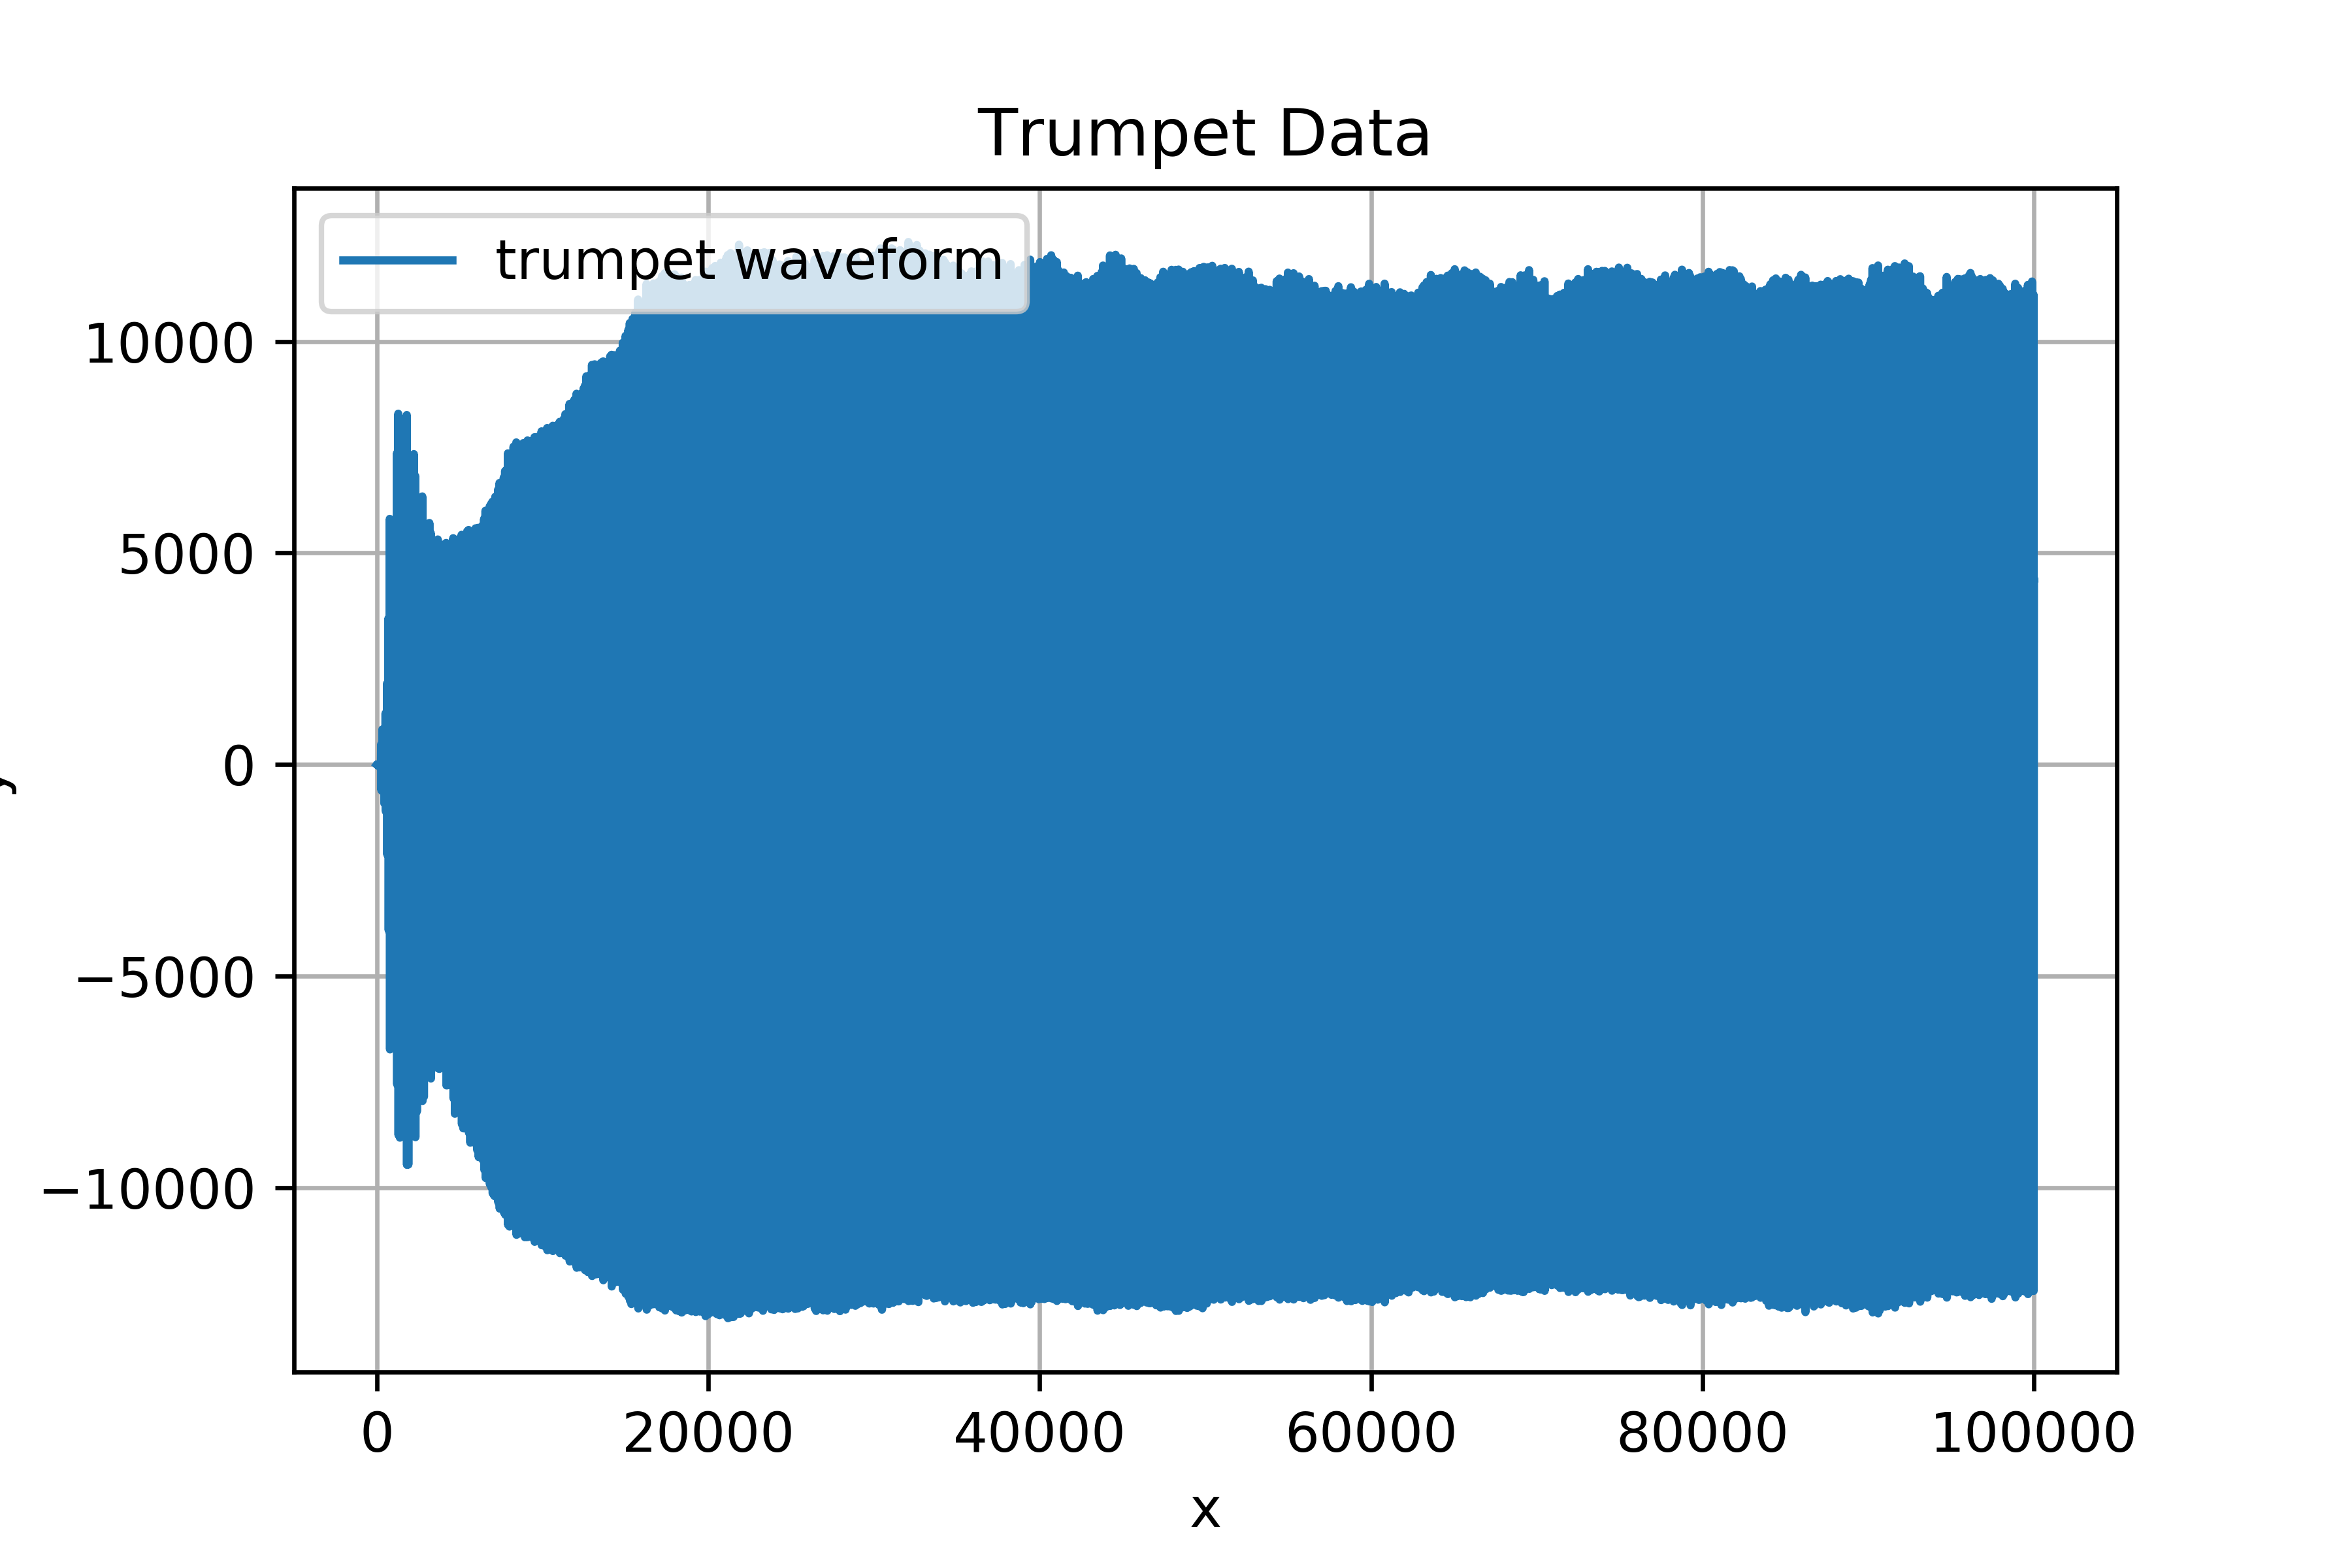
\includegraphics[width=0.8\textwidth]{../images/trumpet_wave.png}
	\caption{Plot of the waveform for a note played on a trumpet, sampled at $44.1kHz$, and provide from the trumpet.txt data file available on the Newman Computational Physics site.}
	\label{fig:trumpet_wave}
\end{figure}

\begin{figure}[H]
	\centering
	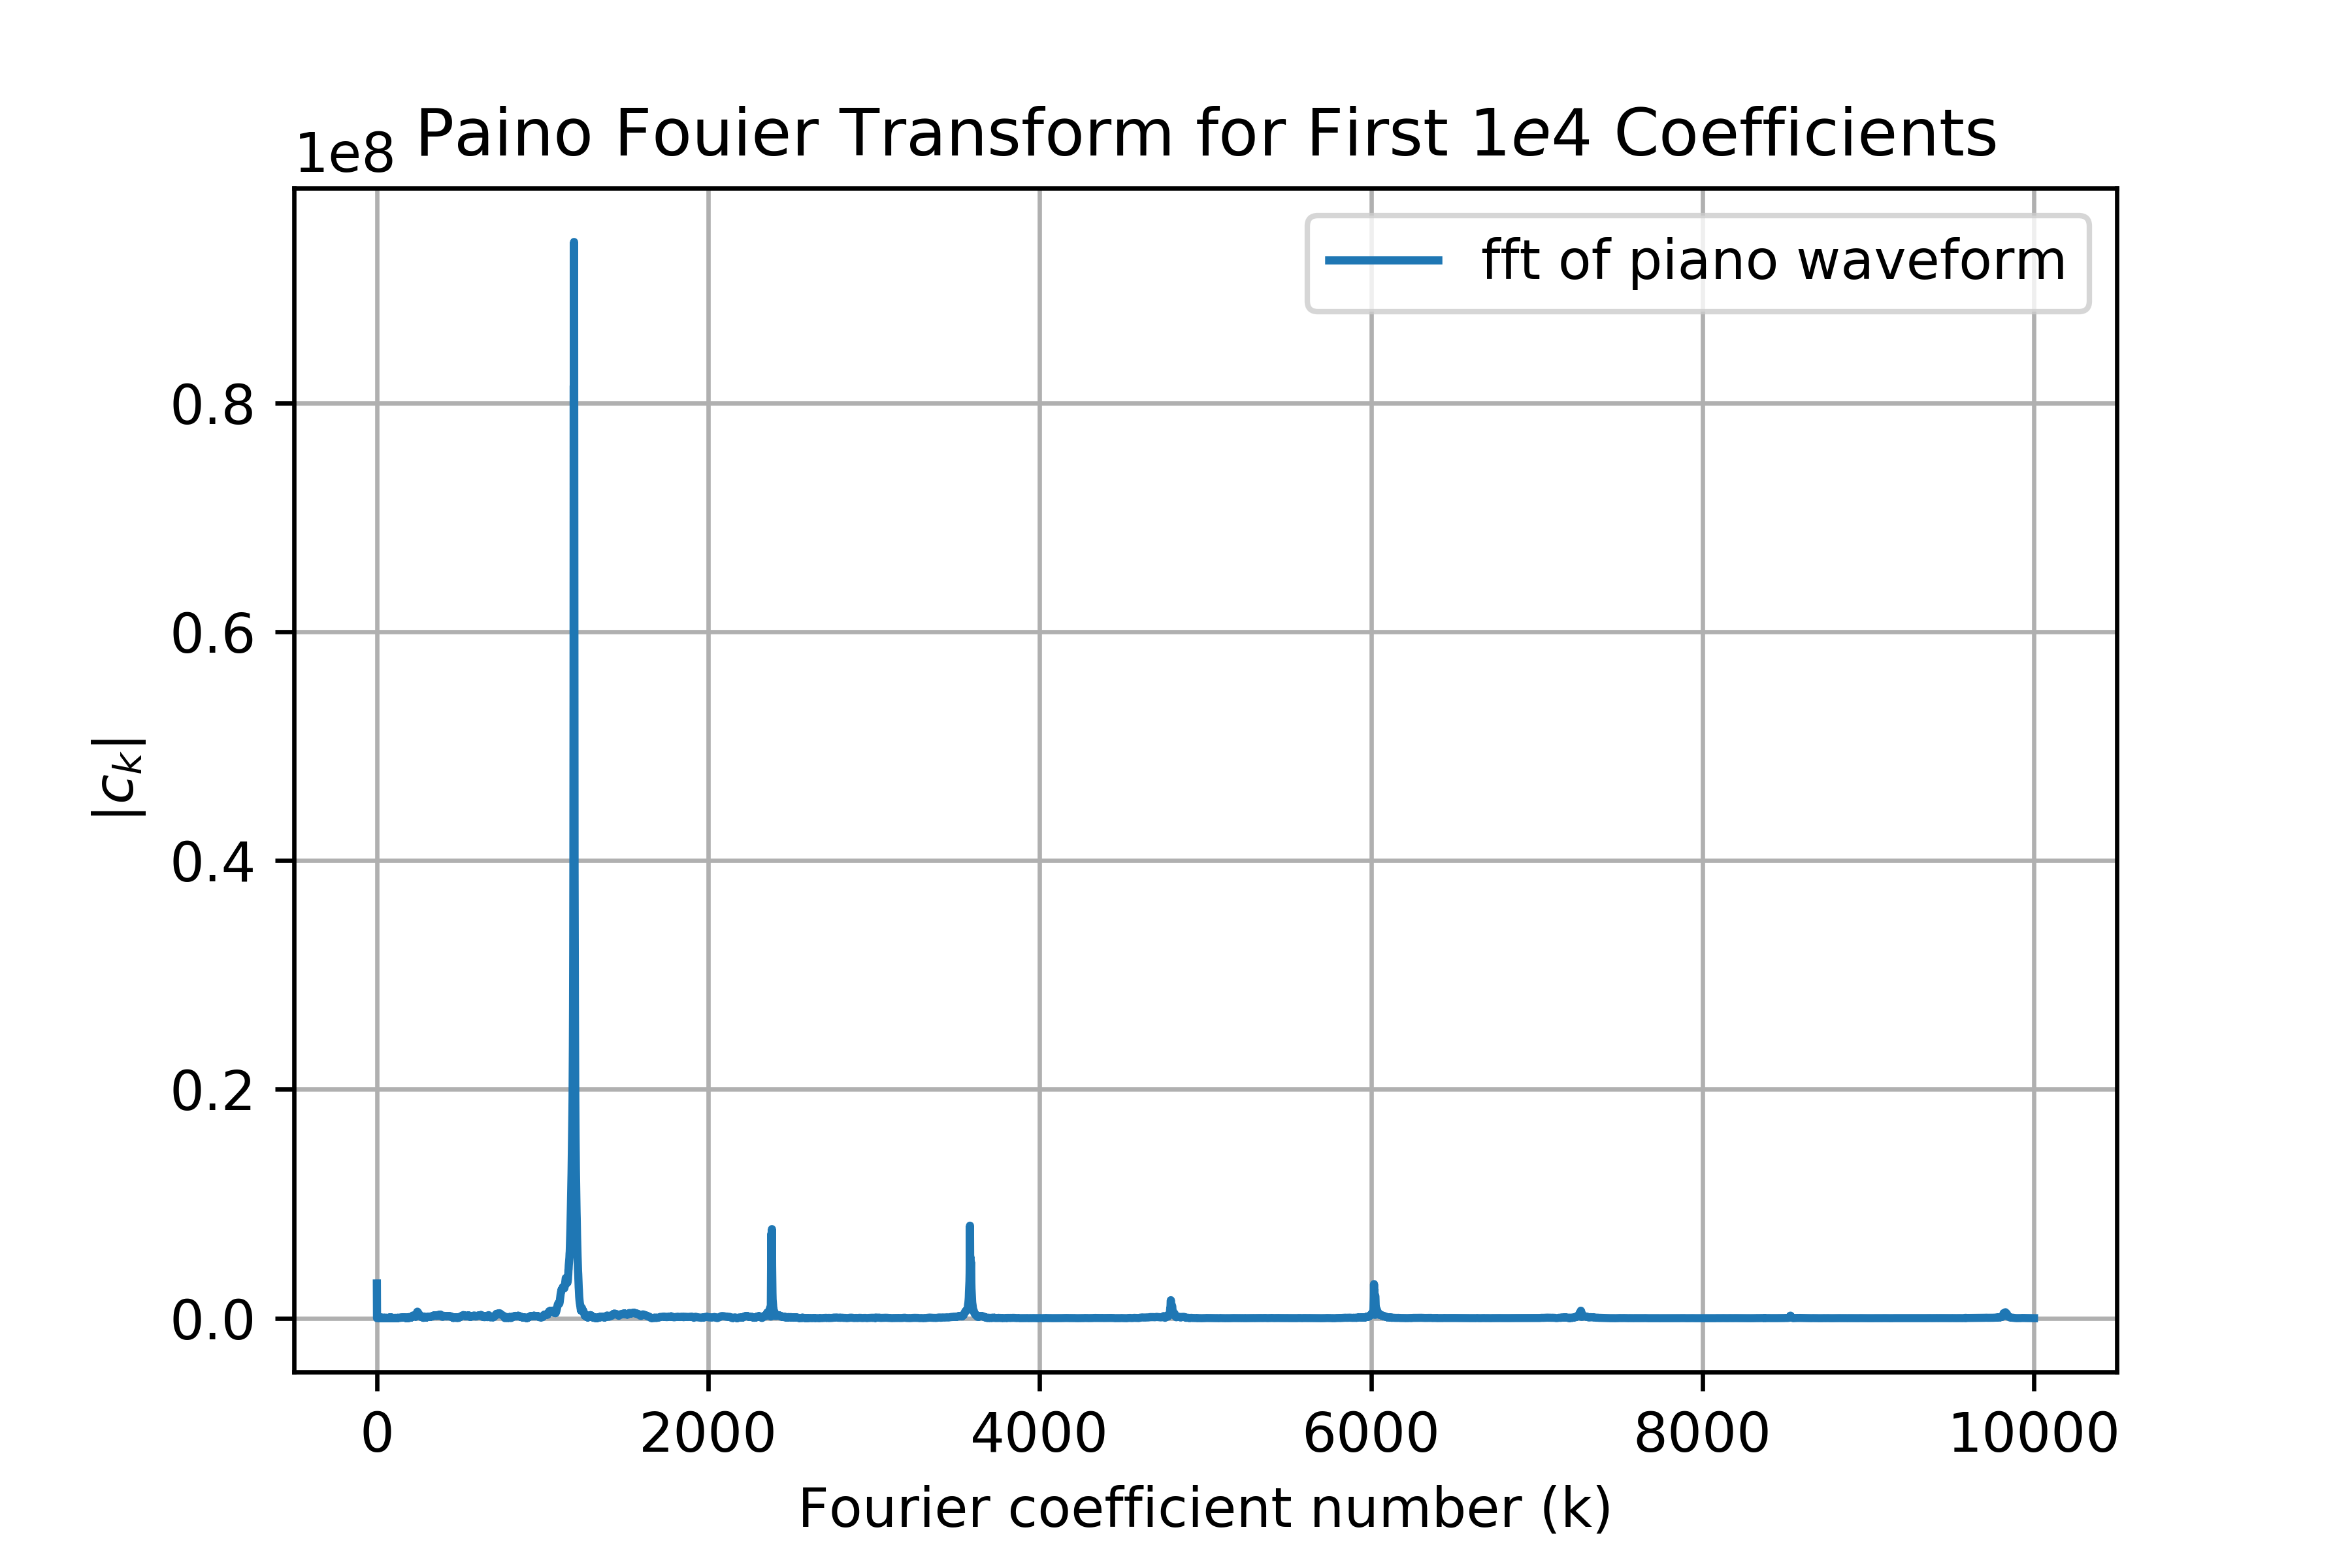
\includegraphics[width=0.8\textwidth]{../images/piano_fft.png}
	\caption{Plot of a Fourier transform of the piano waveform for the first 10,000 coefficients.}
	\label{fig:piano_fft}
\end{figure}

\begin{figure}[H]
	\centering
	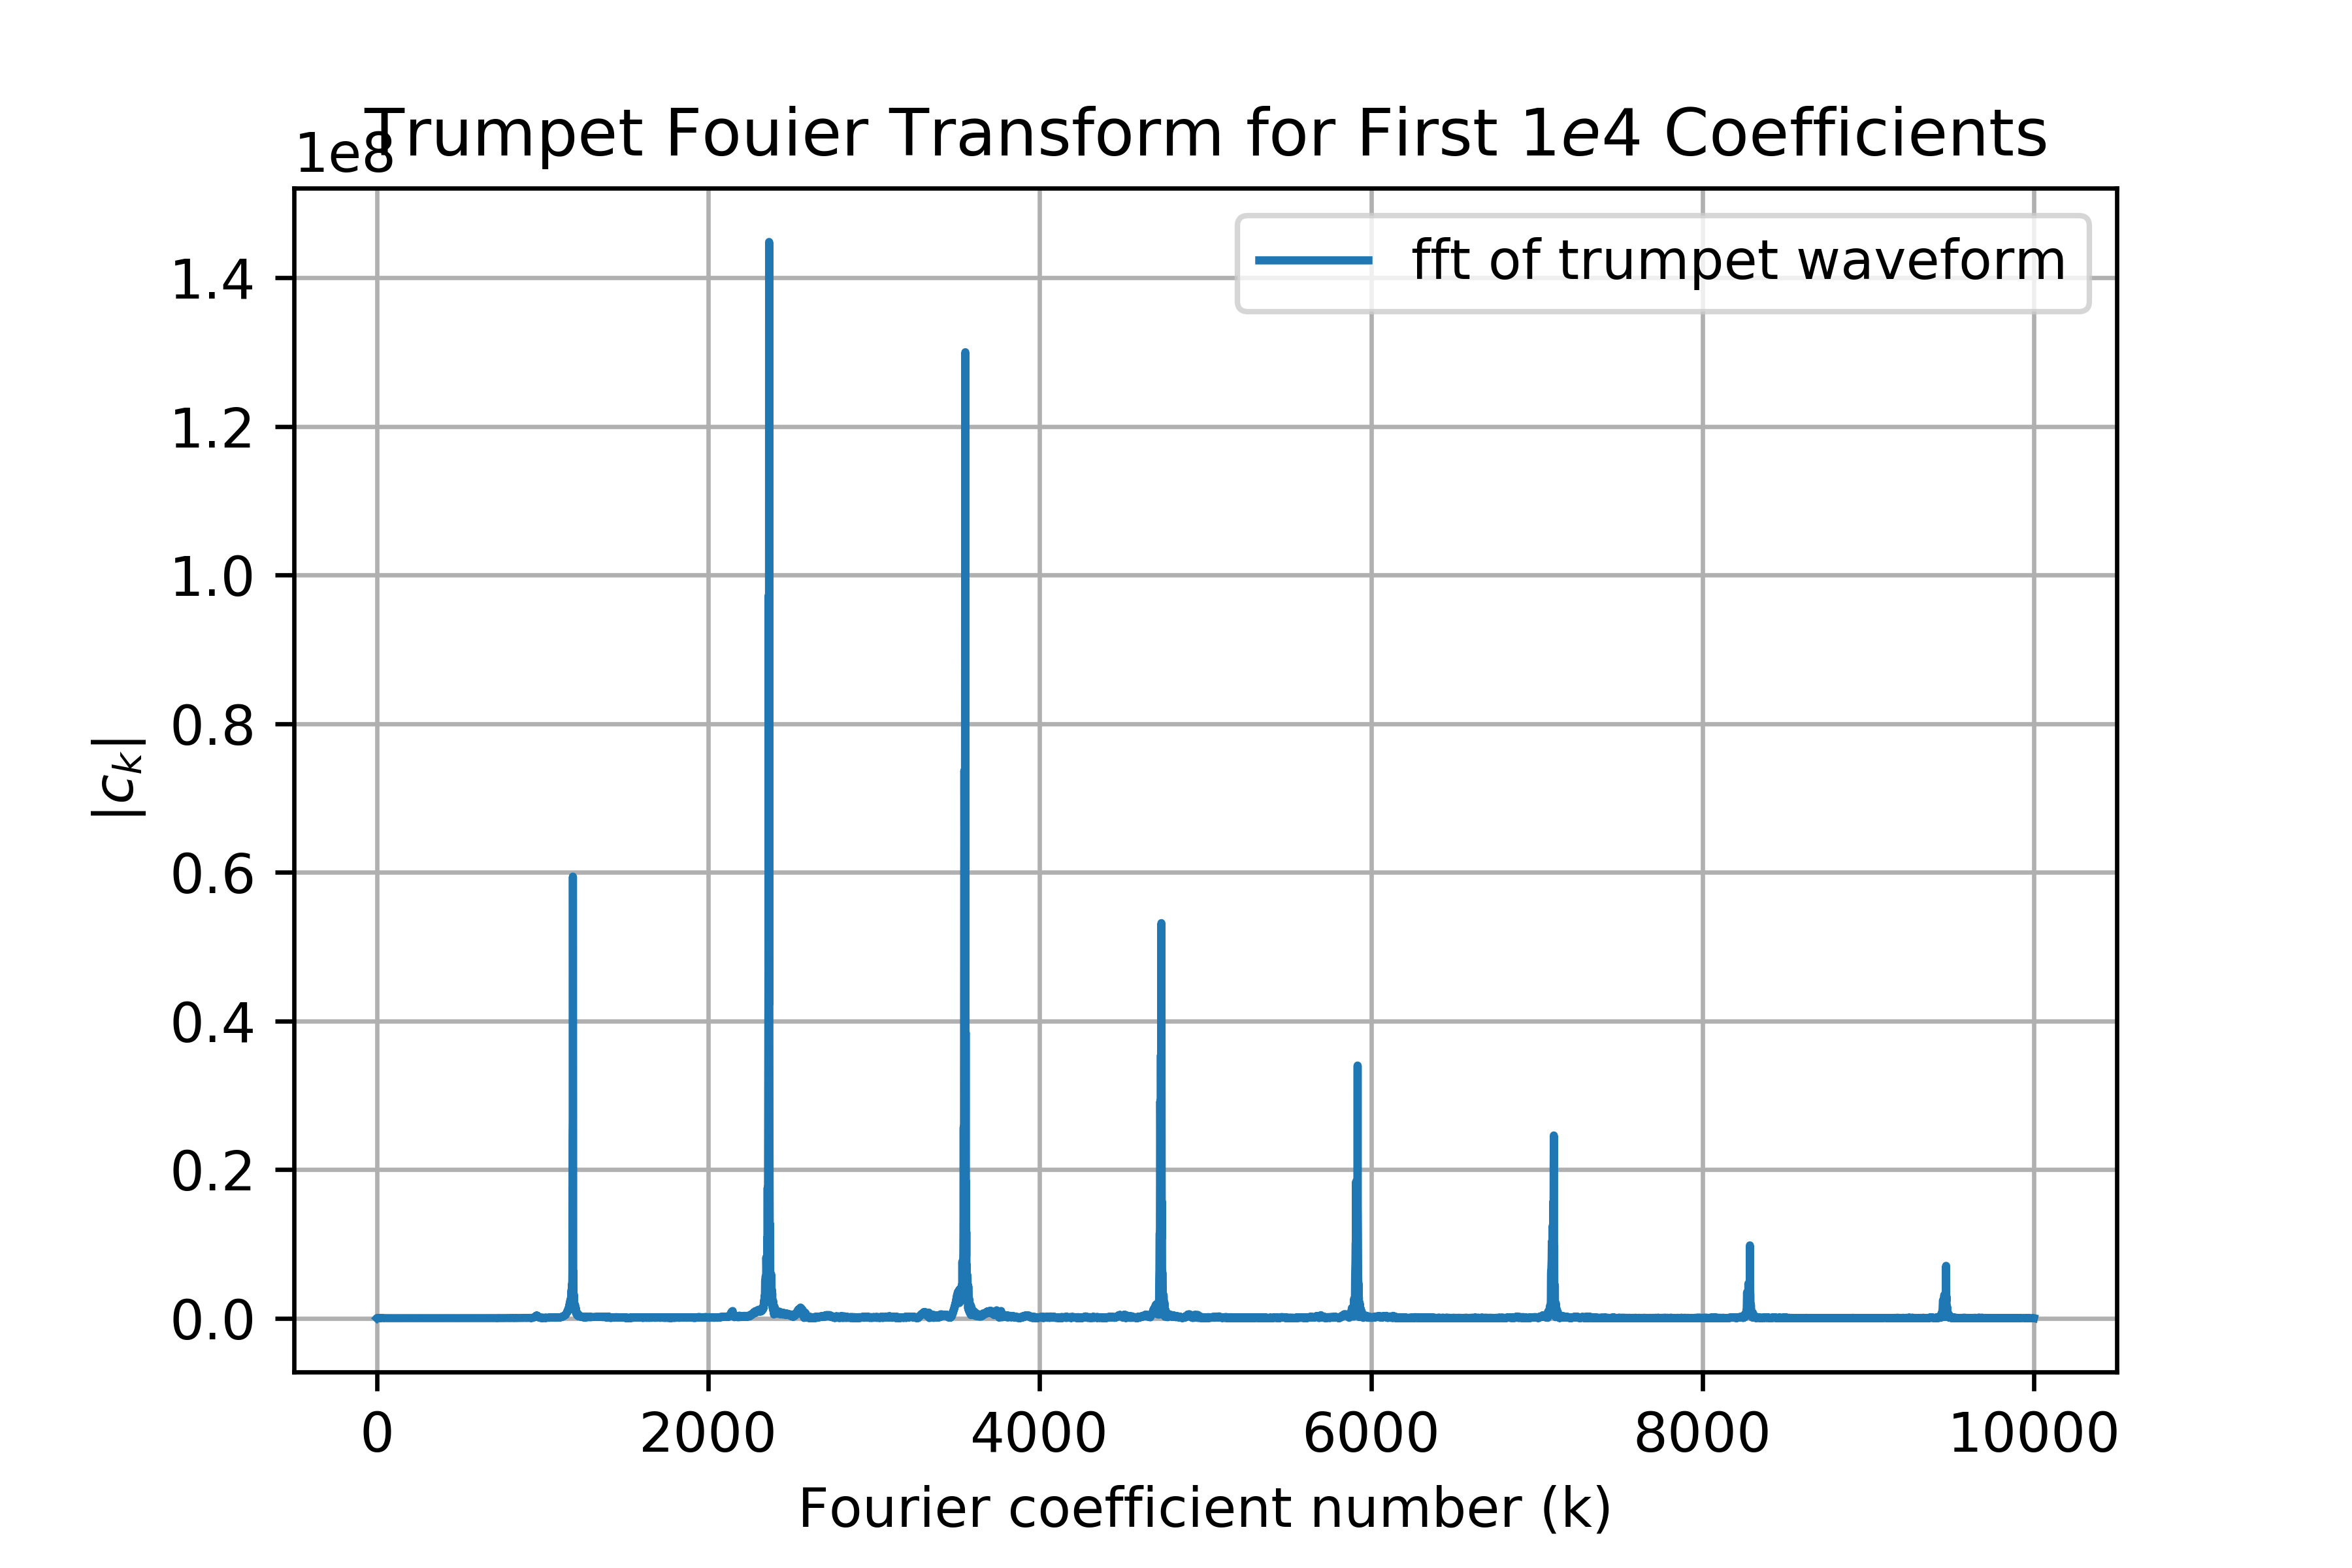
\includegraphics[width=0.8\textwidth]{../images/trumpet_fft.png}
	\caption{Plot of a Fourier transform of the trumpet waveform for the first 10,000 coefficients.}
	\label{fig:trumpet_fft}
\end{figure}

\subsubsection{Part b)}
Given that the waveforms were recorded at a $44.1kHz$ sampling rate, the sampling rate of the Fourier transformed data is halved to $22.05kHz$. The corresponding frequency per bin was then computed in python using

\begin{equation}
	\text{freq per bin of fft} = \frac{\text{fft sample rate}}{\text{number of samples of fft}}
\end{equation}

and getting a value of $0.441$. Using this the coefficient of the largest peaks was then scaled by this frequency per bin to retrieve the frequency of the peaks. The large peak for the piano fft returned a value of $525.672Hz$ and that of the trumpet returned a value of $1044.288Hz$. Since the question mentions that the same musical note was played on both instruments and the piano fft only contains one note it's clear that the peak of the trumpet fft is not the note that was played. Instead taking the first peak we retrieve a value of $521.262Hz$ which matches our result for the piano. Thus the musical note played was $~522Hz$ which is a C note one octave higher than middle C.


\section{Newman 7.9: Image Deconvolution}
The Fourier transform is very useful for filtering out noise from a given data set. Extending this principle to a set of two dimensional data that corresponds to an image, we can perform a deconvolution of the image and output a sharper image. This question does exactly this by computing the Fourier transform of a blurry image and a point spread function, combining the two through the relation $a_{kl} = \frac{b_{kl}}{f_{kl}}$ where $a_{kl}$ is the Fourier transform of the clear image data, $b_{kl}$ is the Fourier transform of the blurry image data, and $f_{kl}$ is the Fourier transform of the point spread function.

\subsection{Part a)}
Using the blur.txt data file from Newman's Computational Physics site, a greyscale density plot of the data is shown in figure \ref{fig:blurred_image}. The image appears with high resolution but out of focus which allows us to sharpen the image via this process.

\begin{figure}[H]
	\centering
	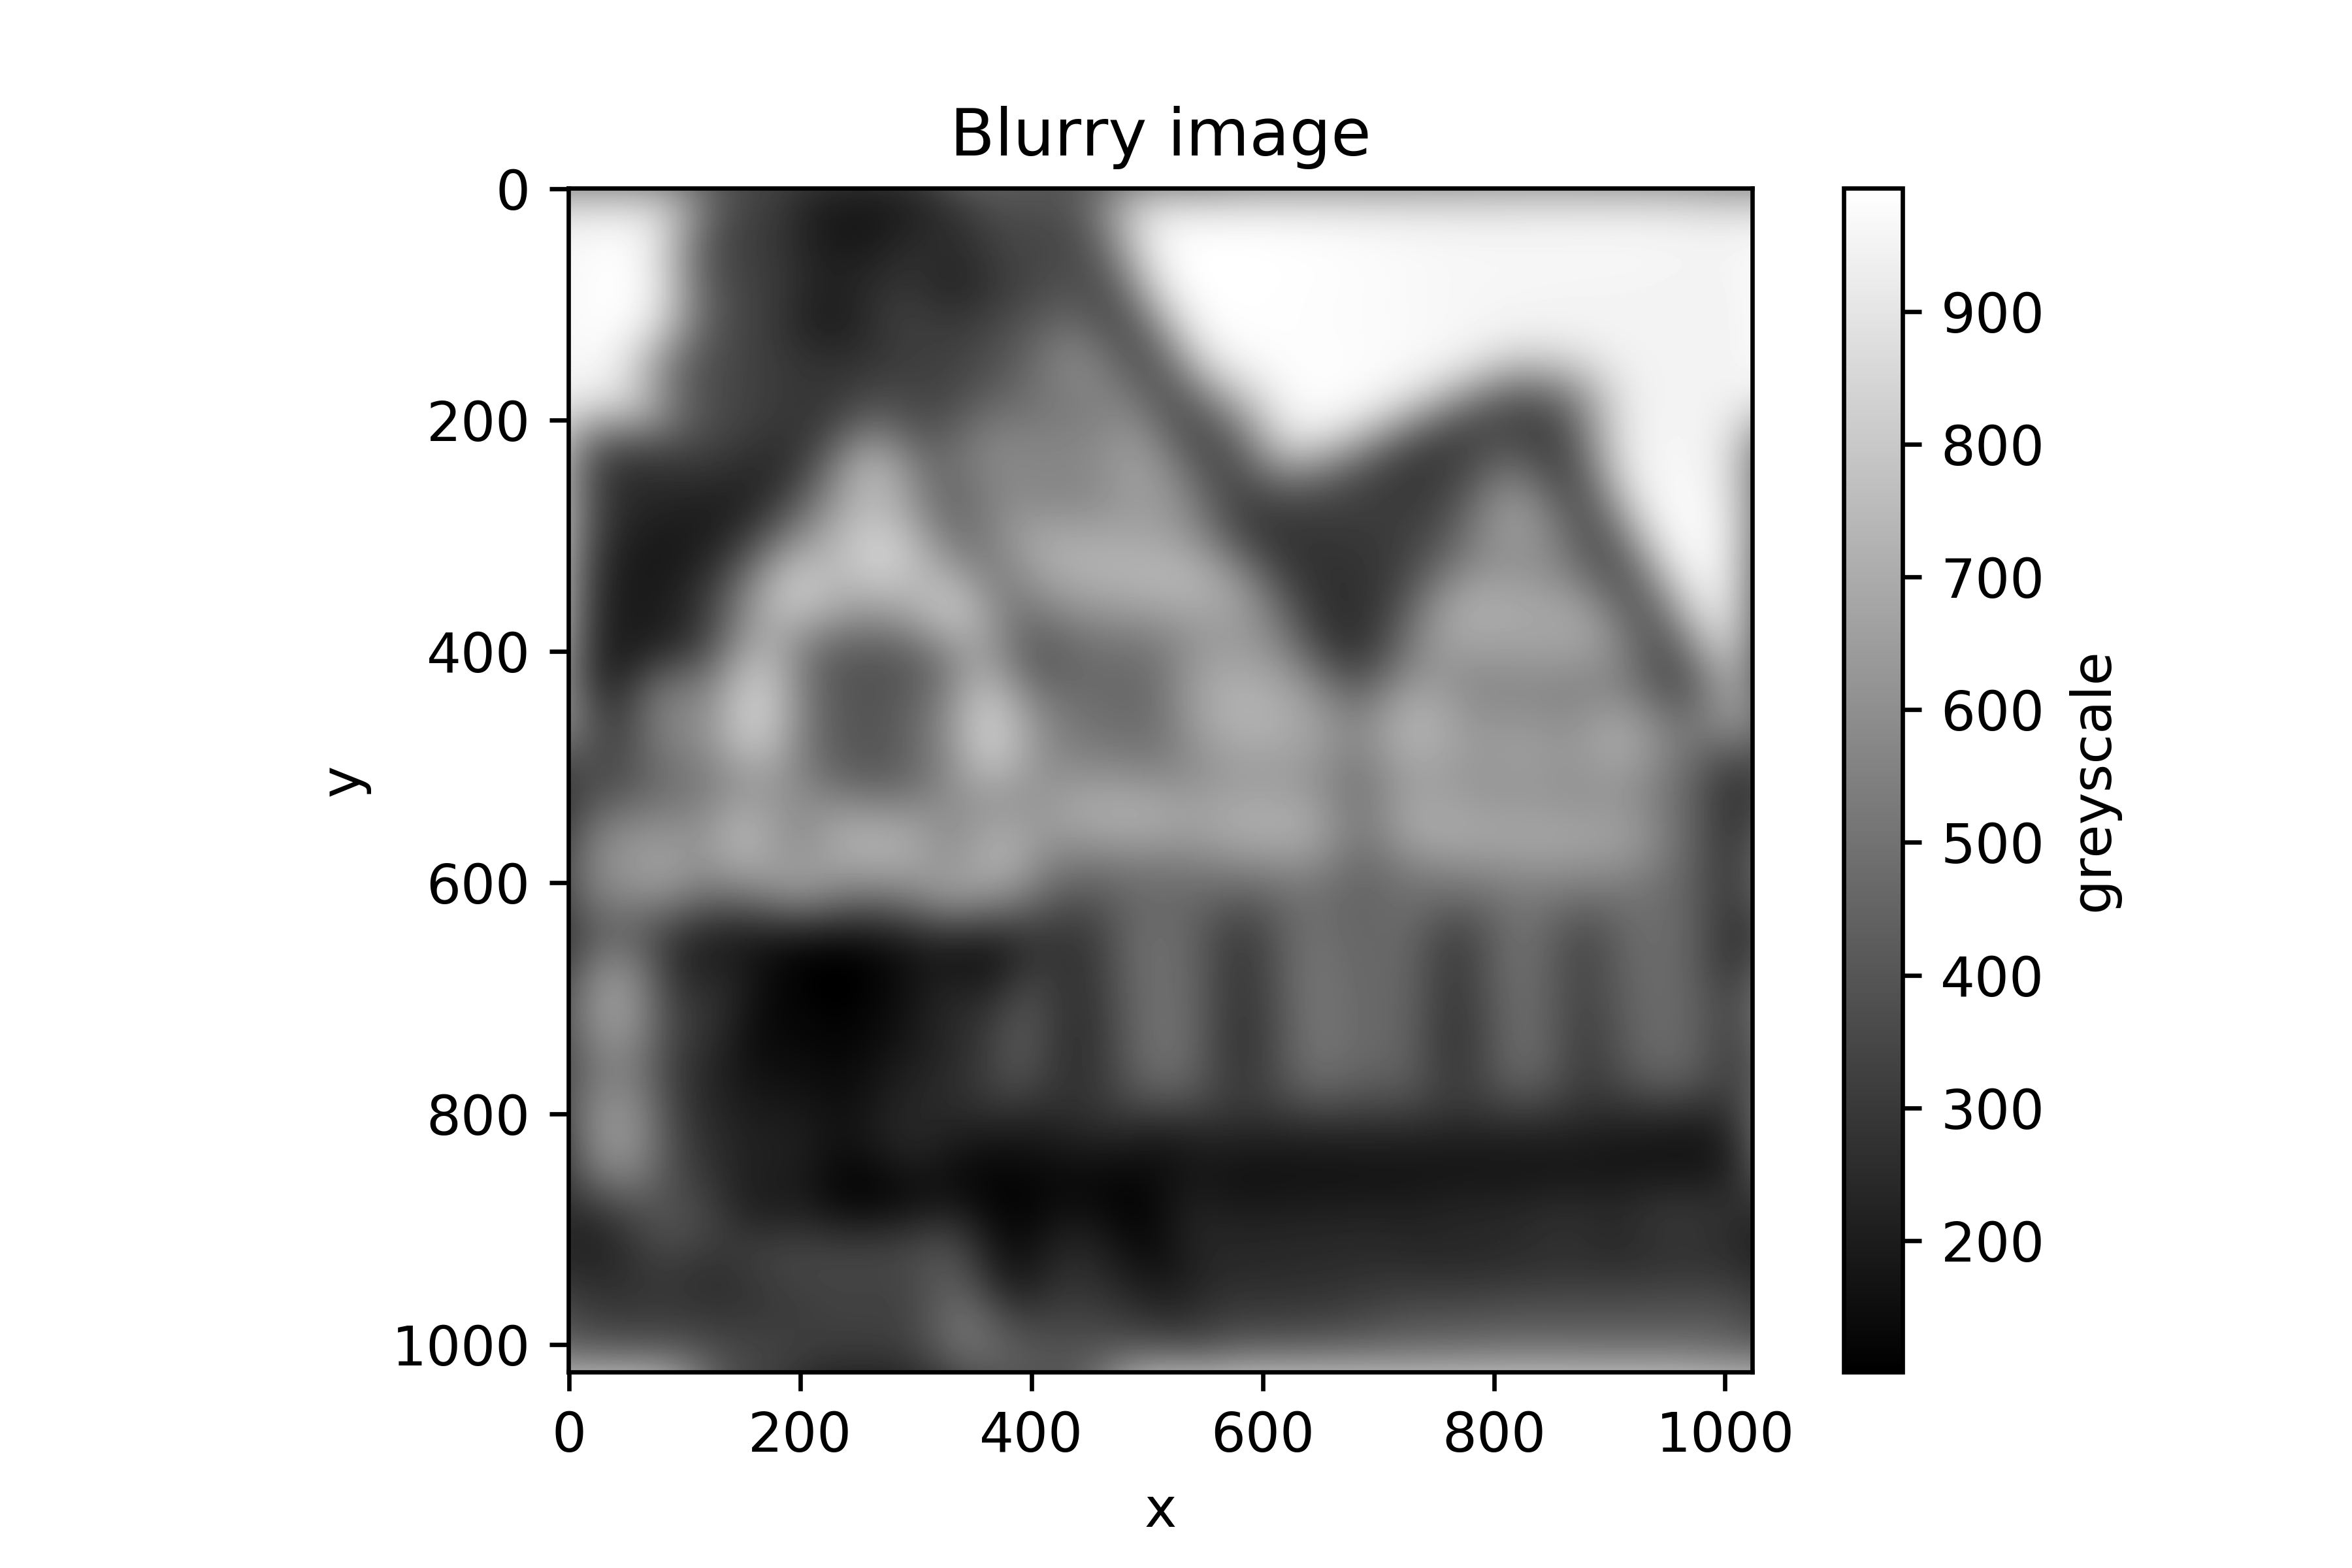
\includegraphics[width=0.8\textwidth]{../images/blurred_image.png}
	\caption{Density plot of provided data shows a blurred image in greyscale.}
	\label{fig:blurred_image}	
\end{figure}

\subsection{Part b)}
The Gaussian point spread function $f(x,y) = exp(-\frac{x^2+y^2}{2\sigma^2})$, periodic in the interval of the original data, was computed for each point of the corresponding blurred image, starting with $(x=0,y=0)$ in the top-left corner. A brightness graph of the spread function is shown in figure \ref{fig:spread_func}.

\begin{figure}[H]
	\centering
	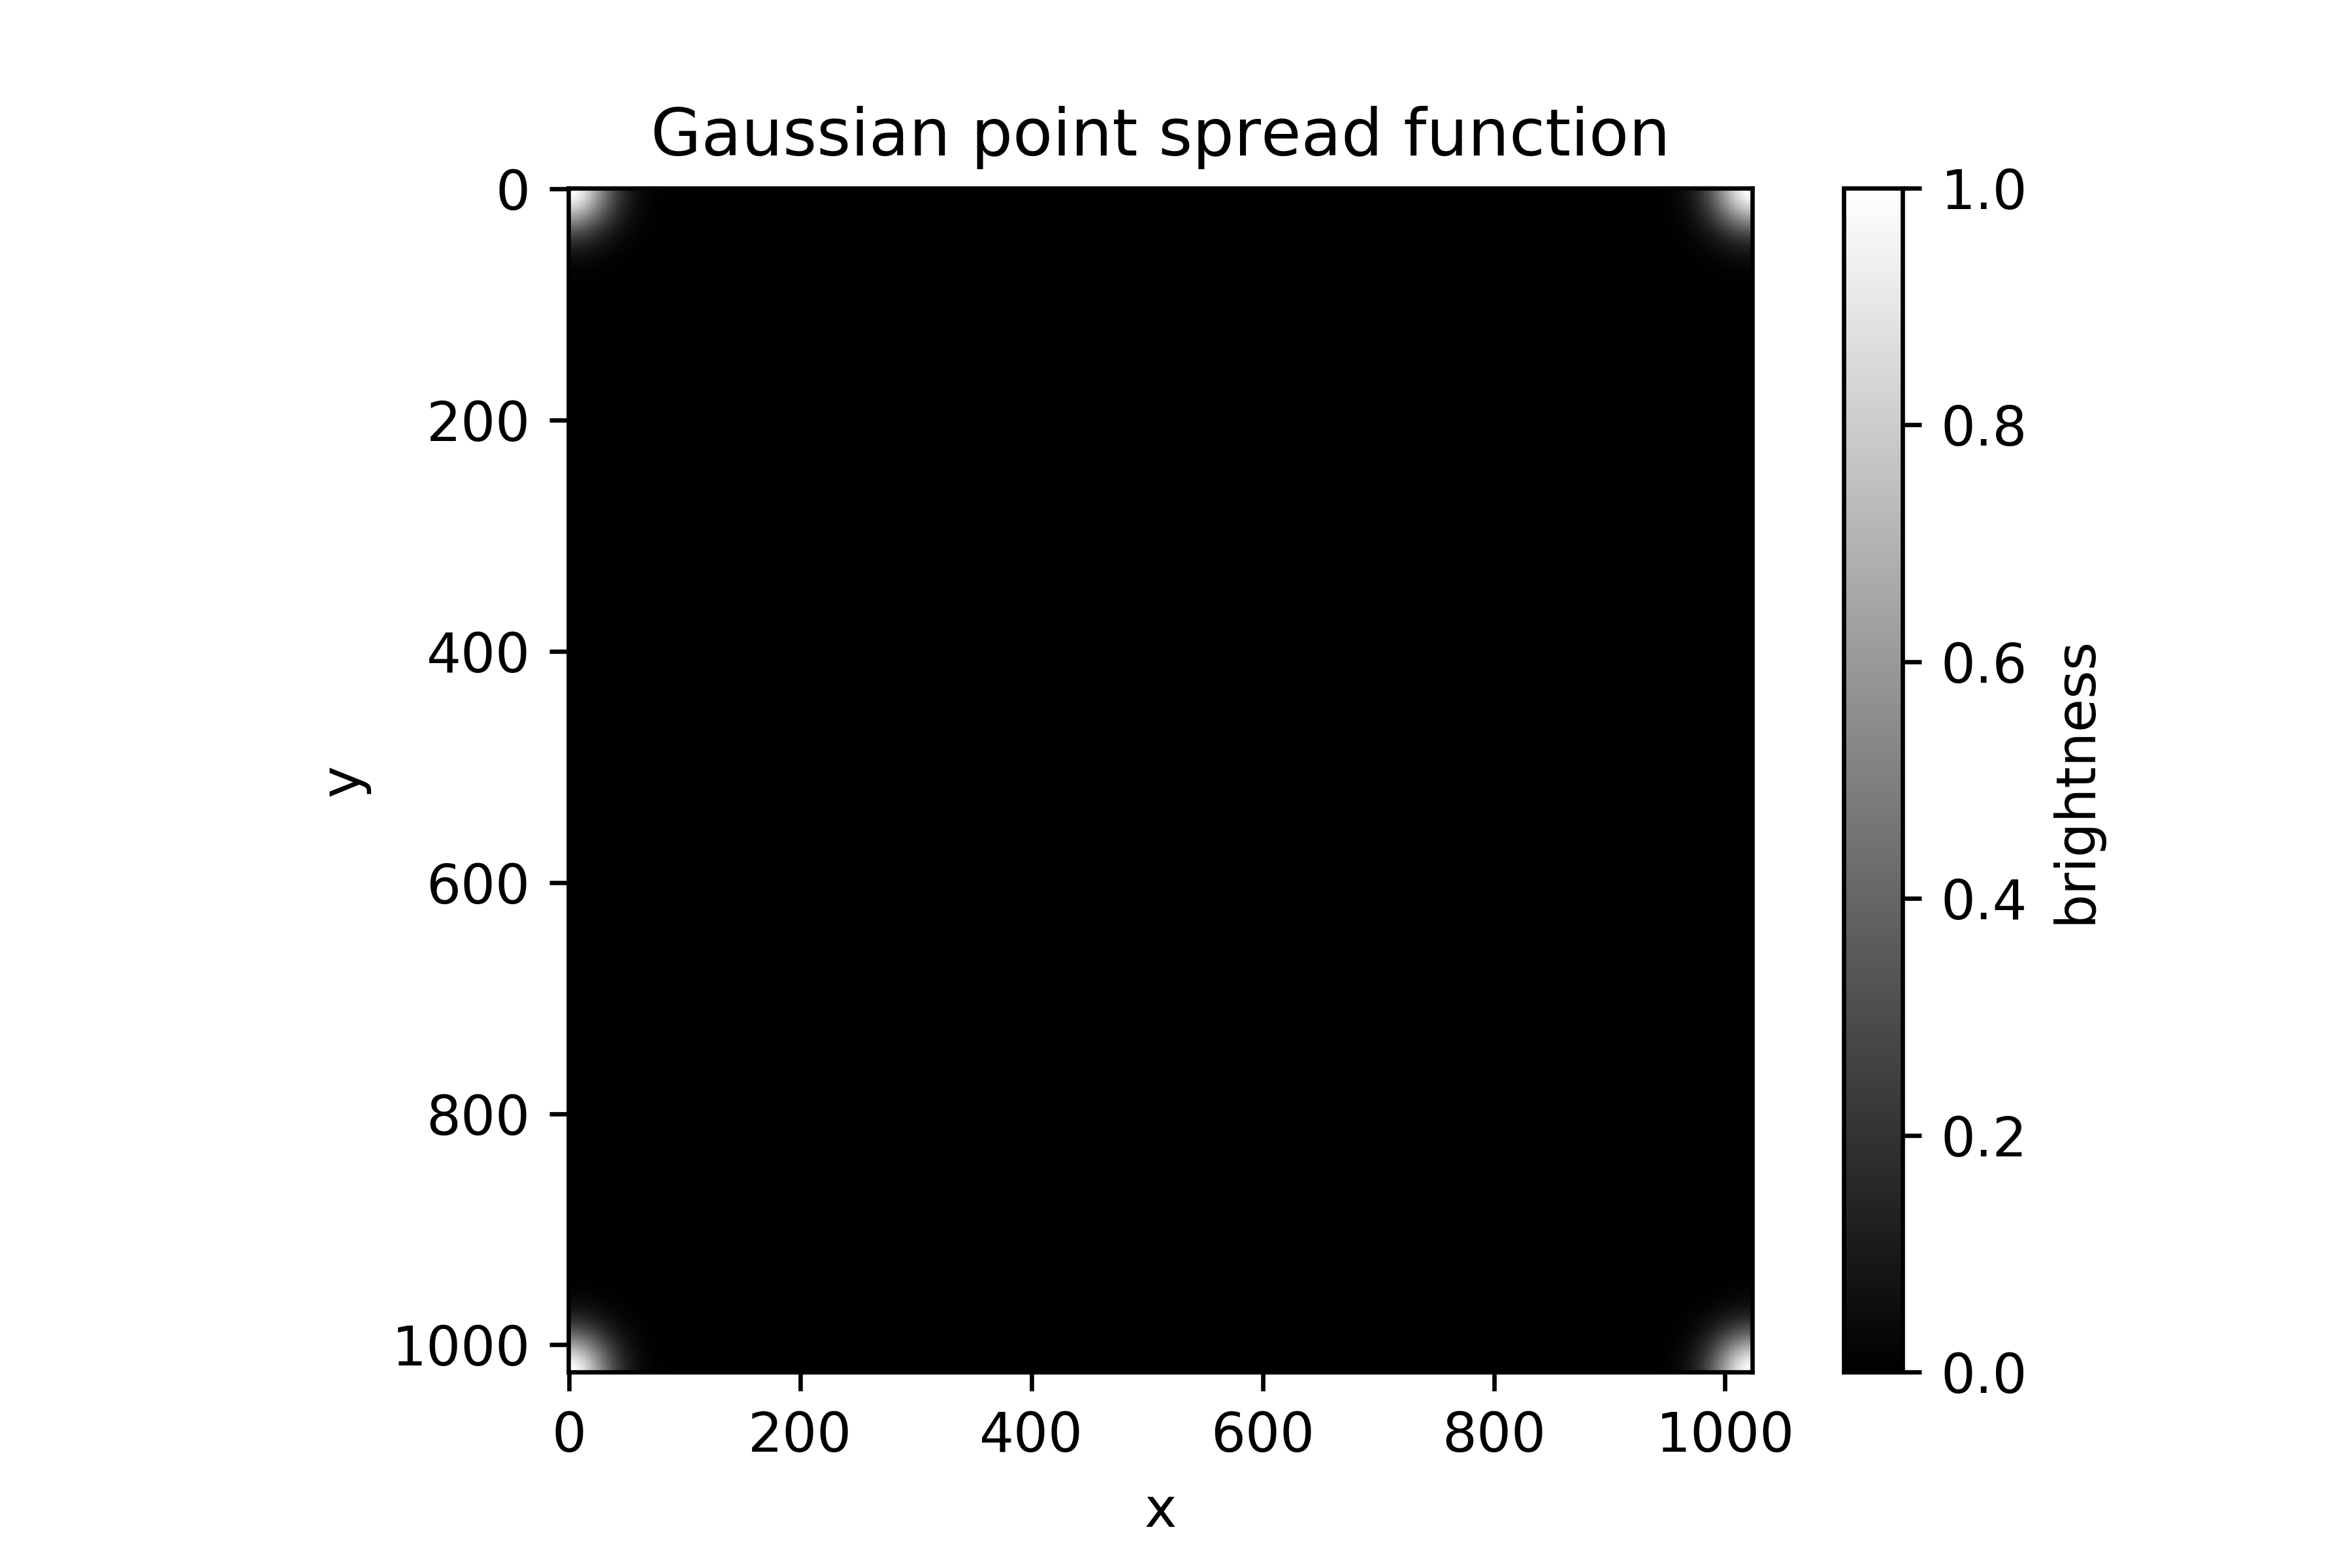
\includegraphics[width=0.8\textwidth]{../images/spread_function.png}
	\caption{Plot of the Gaussian point spread function with $\sigma=25$ used to sharpen the image.}
	\label{fig:spread_func}	
\end{figure}

\subsection{Part c)}
Using the results from part a) and b) we applied a Fourier transform, using the numpy function rfft2, to both the blurred image data set and the spread function data set.
The fft of the blurred image was then divided by the fft of the spread function as described above. To account for the small and possibly zero valued entries in the spread function data set, a cutoff value of $10^{-3}$ was used (wherein the spread function was not applied if the entry values was below the cutoff). Additionally, the textbook notes that the blurred data set should also be divided by the dimensions of the data set, however providing this additional factor resulting in a failure of the deconvolution.
The adjusted fft data was then pass through the inverse, irfft2, function to retrieve a sharpened data set of the original image, which has been graphed in the density plot shown in figure \ref{fig:deconvolved_image}. The resulting image still contains some noise within it however we can now clearly see that the original image was taken of a house with a couple of people walking by in front of it. 

\begin{figure}[H]
	\centering
	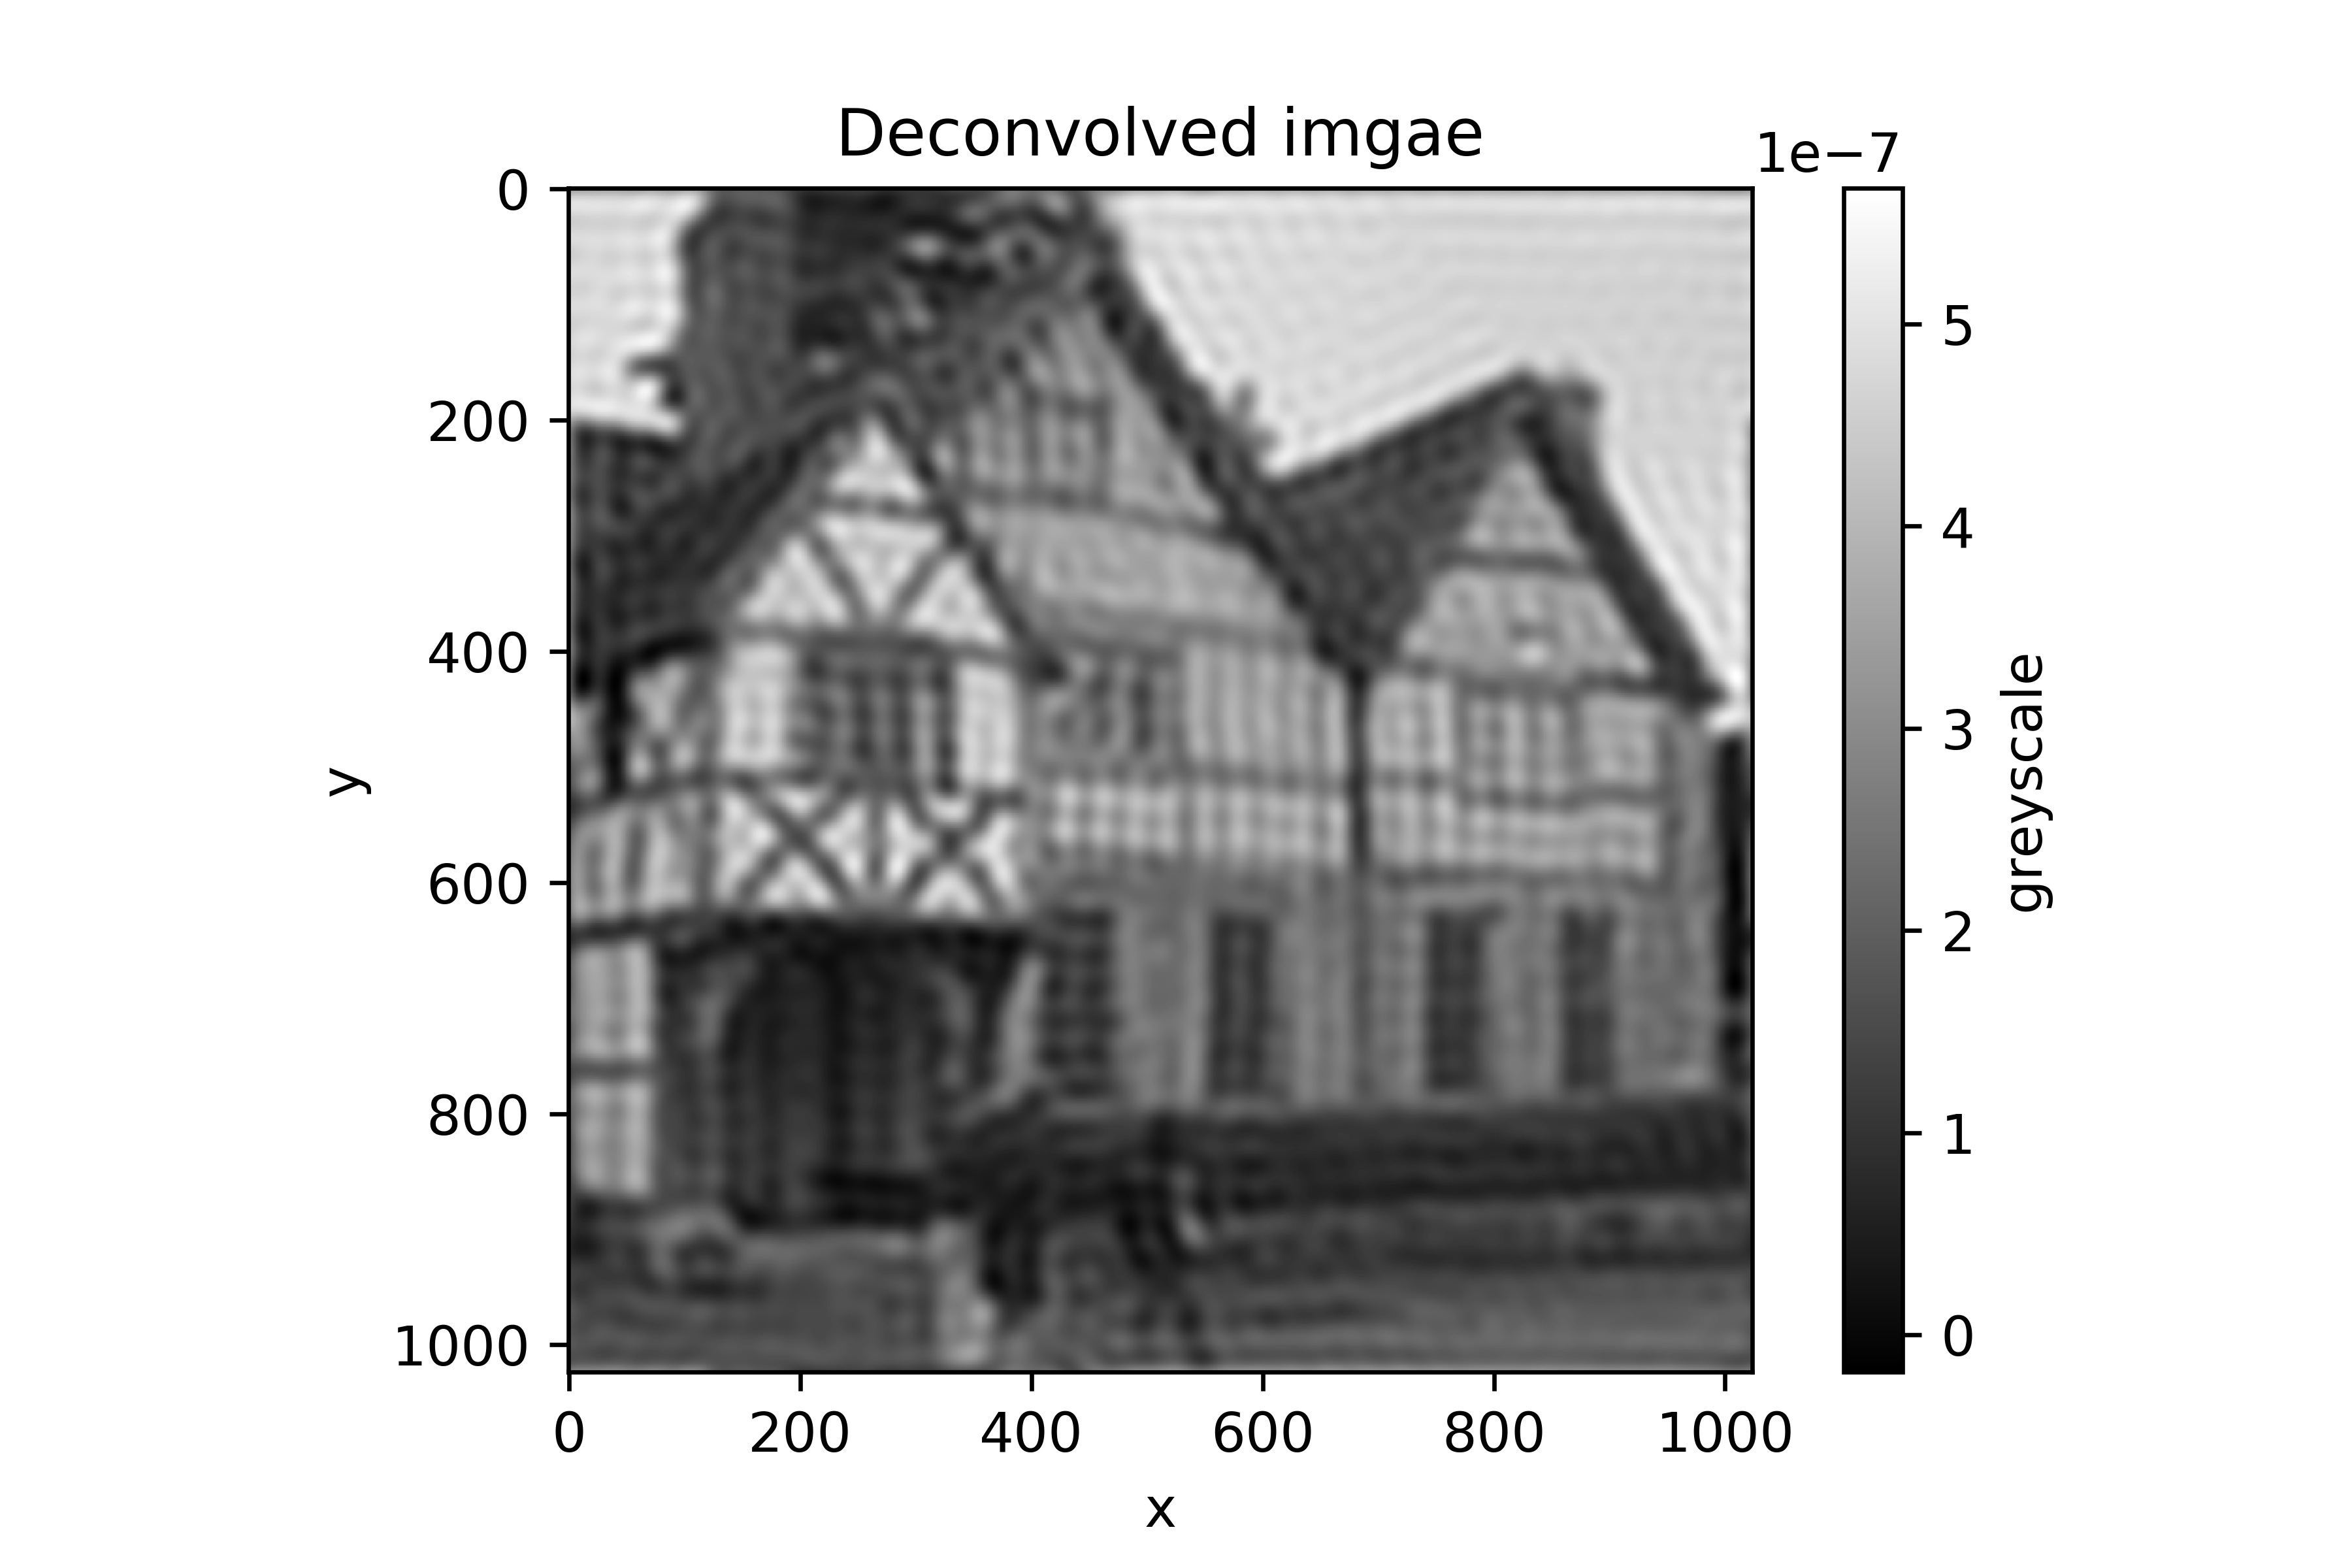
\includegraphics{../images/deconvolved_image.png}
	\caption{Density plot of the greyscale image after applying the spread function via Fourier transform.}
	\label{fig:deconvolved_image}	
\end{figure}

\end{document}